\chapter{He Made \$500 Million Playing Real Life Monopoly}

In this School of Hard Knocks interview, curated by LazyingArt LLC, the lesson arrives in two stages. First comes the teaser: a man worth roughly half a billion dollars, a mansion named first at \$20 million and later corrected to \$30 million, and the promise that we are about to see how real-estate wealth is built. Then the scene resets, the host calls the conversation a ``master class,'' and the lecture proper begins. We are not given a blackboard proof. We are given something narrower and, in its own way, just as instructive: an arithmetic of leverage, margin, and repetition.

\section{Cold Open, Reset, and the Promise of Method}

The opening numbers are there to create scale before they create understanding. We are supposed to feel the distance between ordinary means and the world into which the interview is stepping. Only after that distance has been established does the host tell us what question will actually govern the chapter: how does one create wealth through real estate in today's world, even without much starting money?

The framing quantities are simple:
\begin{align}
W &\approx \$500\,\text{million},\\
M &\approx \$20\,\text{million}\qquad \text{(cold-open claim)},\\
M &\approx \$30\,\text{million}\qquad \text{(later spoken correction)}.
\end{align}
These are not worked results. They are narrative instruments. They justify why the conversation matters and why the host can recast the meeting as a lesson rather than a tour of somebody else's lifestyle.

That reset matters. The host moves from ``look at this place'' to ``this is going to be a master class,'' and Ben Mala accepts the frame with the half-joking line that he is the master and the host the student. Once that authority transfer is complete, the interview can stop displaying outcomes and start unpacking the machinery that produced them.

\section{Why Real Estate?}

The first serious move is not numerical. It is definitional. Mala is asked about background, and the answer is not inherited money but poverty. He then moves quickly from biography to principle: real estate is common because it is tied to ordinary need. People need places to live, to work, and to shop. In that sense, the asset class is introduced first as infrastructure and only second as a vehicle for accumulation.

\subsection{Question \& Answer}

\paragraph{Question.} Why real estate rather than some other route to money?

\paragraph{Answer.} Because, in the logic of the lecture, real estate sits underneath daily life. It is not presented as fashionable or exotic. It is presented as necessary. That is why the speaker can begin with affordable housing, move to retail, and then to hotels without changing the underlying thesis. The forms differ, but the demand basis remains.

This is the first anchor of the chapter. We are not yet being taught leverage. We are being taught why leverage, if used at all, is being applied to something with durable use.

\section{Borrowing Is the First Move}

Once the conversation turns from background to hotels, the lecture sheds a common beginner's fantasy. If we do not have money, we do not wait passively for money to appear. We learn to borrow against a property that supports borrowing.

The host asks how hotels are bought. The answer comes in the order of operations: the hotel makes money, the bank looks at it, the property is appraised, and financing enters if the deal makes sense. In a cautious reconstruction, the speaker's ``eighty cents on the dollar'' has the form
\begin{equation}
D \approx 0.8P,\qquad E \approx 0.2P,
\end{equation}
where $P$ is purchase price, $D$ lender debt, and $E$ investor equity.

We should read this as a colloquial loan-to-value claim, not as a universal underwriting law. The real point is structural. Most of the capital may come from the lender if the asset itself can justify it.

\subsection{Question \& Answer}

\paragraph{Question.} Do we need our own money to get started?

\paragraph{Answer.} Not necessarily. The lecture's answer is that we need a deal that can be financed and a position from which the bank can say yes. The problem is not ``How do we avoid debt?'' The problem is ``How do we place debt against the right asset?''

This is where the rhythm of the interview sharpens. The host keeps pressing from generalities to mechanism. ``How do you get the money?'' ``Where do you borrow?'' ``Will a bank lend if you have no capital?'' The repeated forcing function is useful: it keeps the lecture from floating away into slogans.

\section{First Steps: VA, FHA, and the Fourplex Logic}

The lecture now steps down from hotels to the smallest plausible beginner's ladder. This is important. It would be easy to leave the discussion at the scale of large properties and imply that the listener must already be in the game at size. Instead, the speaker gives specific entry routes for a low-capital investor.

For a VA path, the lecture presents the down payment as essentially zero:
\begin{equation}
E_{\mathrm{VA}} \approx 0.
\end{equation}
For FHA, the lecture gives a definite fraction:
\begin{equation}
E_{\mathrm{FHA}} = 0.035P.
\end{equation}
Both routes are attached to one-to-four-unit properties. That is the first real beginner's mechanism in the interview.

The four-unit property is then turned into a simple cash-flow arrangement. We occupy one unit and rent the remaining three. If $R_2,R_3,R_4$ denote the rents from the other units and $C$ the total carrying cost in a schematic sense, then the lecture's logic is
\begin{equation}
R_2+R_3+R_4 \geq C.
\end{equation}
If the inequality is stronger,
\begin{equation}
R_2+R_3+R_4 > C,
\end{equation}
then the owner is not merely carried; the owner may live in unit $1$ and still generate positive cash flow.

We should be careful here. ``Live for free'' and ``the three units will pay all your bills'' are target economics, not guarantees. They depend on the purchase being right. That is why the lecture keeps returning to the phrase ``it's all in the buy.'' The carrying structure is not magic. It is a consequence of price discipline.

\begin{enumerate}
\item Choose a financing structure that permits low entry equity.
\item Stay within a one-to-four-unit category.
\item Occupy one unit.
\item Rent the others.
\item Require the rent stream to cover the carrying cost.
\item Only then do we get the celebrated beginner's outcome.
\end{enumerate}

This is the chapter's first genuinely worked ladder. It is not abstract advice. It is procedure.

\section{Debt, Rates, and the Cushion in the Deal}

Now the interview raises the objection that every beginner raises sooner or later: debt feels dangerous. The reply is not to deny the feeling. It is to force the feeling into arithmetic.

\subsection{Question \& Answer}

\paragraph{Question.} Is debt itself the danger, or is a thin deal the danger?

\paragraph{Answer.} The interview argues for the second. Debt is an instrument. What matters is whether the deal has enough margin to carry debt without being destroyed by ordinary financing costs.

The speaker's cleanest capital-stack example is a \$10 million deal:
\begin{equation}
P = E + D = \$2\,\text{million} + \$8\,\text{million} = \$10\,\text{million}.
\end{equation}
The rhetorical force of the example is obvious: a relatively small slice of investor capital controls a much larger asset. That is the attraction of leverage.

But the chapter does not stop there. It immediately turns to the price of debt itself.

\paragraph{Worked example.} Suppose we borrow
\begin{equation}
D = \$1{,}000{,}000
\end{equation}
at an annual rate
\begin{equation}
r = 0.06.
\end{equation}
Then the yearly interest is
\begin{align}
I_{\text{year}} &= rD = 0.06\cdot \$1{,}000{,}000 = \$60{,}000,\\
I_{\text{month}} &= \frac{I_{\text{year}}}{12} = \$5{,}000.
\end{align}
This is the interview's most explicit numerical check. Once we have the \$5,000-per-month burden in hand, the speaker's qualitative conclusion follows immediately: if the difference between success and failure is whether the rate is $4\%$, $5\%$, $6\%$, or $7\%$, then the transaction was probably too weak from the beginning.

In our notation, the lecture's margin principle is
\begin{equation}
\Pi_{\text{deal}} - I - \text{other costs} > 0,
\end{equation}
with enough cushion that ordinary rate variation does not wipe out the profit. This is a deliberately modest reconstruction; the lecture does not provide a full underwriting model, and we should not pretend that it does.

The line ``the bank takes all the risk'' should also be read carefully. It is not a literal decomposition of downside exposure. It is leverage rhetoric. Still, its teaching function is clear: the investor is being trained to think in terms of controlled equity, asset support, and asymmetry rather than in terms of paying cash for everything.

\section{An Editorial Break, Then a Move to Scale}

At this point the interview is interrupted by a host-read promotion for mentorship and community. That interruption should be visible in the notes because it alters the rhythm: for a stretch, we leave Mala's method and enter the channel's business model. When the interview resumes, it does not return to the beginner's ladder. It returns at a larger scale and asks what the business looks like once the investor is already moving real assets.

The first result is a hotel repositioning example. A hotel is bought for \$17 million, roughly \$6 million is put into fixing it up, and the finished property is later sold for \$34 million. The rough gross spread is therefore
\begin{equation}
\Pi_{\text{gross}} \approx \$34\,\text{million} - \bigl(\$17\,\text{million} + \$6\,\text{million}\bigr) = \$11\,\text{million}.
\end{equation}
The lecture stresses another important point here: the improvement money is said to come from hotel operations rather than directly from the owner's pocket. Even in this large example, operating cash flow and capital structure remain central.

\subsection{Question \& Answer}

\paragraph{Question.} What should we buy, given the amount of money we actually have?

\paragraph{Answer.} The lecture's answer is explicitly scale-dependent. At the top end, data centers are named as the future of real estate: concrete buildings full of computers, dense with power and cooling demand, leased by firms that need digital infrastructure. For the smaller investor, the recommendation changes. The safer first move is residential income property.

The chapter then returns to a concrete small-investor example. Start with \$100,000 of equity. Suppose pre-qualification supports a \$400,000 loan. Then total buying power becomes
\begin{align}
\$100{,}000 + \$400{,}000 &= \$500{,}000,\\
D &= 4E.
\end{align}
If such a \$500,000 building can be improved into something worth
\begin{equation}
V_{\text{after}} \approx \$700{,}000\text{ to }\$800{,}000,
\end{equation}
then the investor has created a larger base against which new borrowing may be supported.

At this point the lecture gives its preferred scaling mechanism: refinance rather than simple liquidation. In a careful schematic reconstruction,
\begin{equation}
\text{Cash Out} \approx D_{\text{new}} - D_{\text{old}}.
\end{equation}
That is, once the asset is worth more, a new loan may exceed the old balance, and the difference becomes deployable capital for the next purchase.

\begin{figure}[h]
\centering
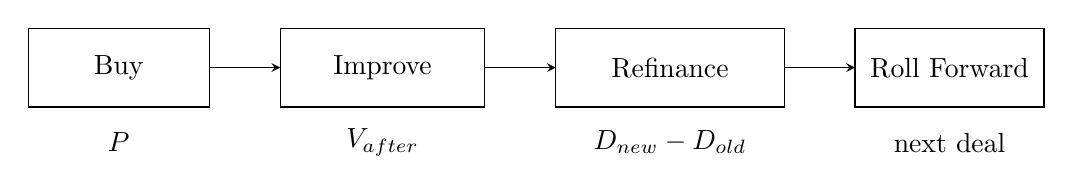
\begin{tikzpicture}[x=1cm,y=1cm,>=stealth]
\draw (0,0) rectangle (2.3,1) node[pos=.5]{Buy};
\draw (3.2,0) rectangle (5.8,1) node[pos=.5]{Improve};
\draw (6.7,0) rectangle (9.6,1) node[pos=.5]{Refinance};
\draw (10.5,0) rectangle (12.9,1) node[pos=.5]{Roll Forward};
\draw[->] (2.3,0.5)--(3.2,0.5);
\draw[->] (5.8,0.5)--(6.7,0.5);
\draw[->] (9.6,0.5)--(10.5,0.5);
\node at (1.15,-0.45) {$P$};
\node at (4.5,-0.45) {$V_{\text{after}}$};
\node at (8.15,-0.45) {$D_{\text{new}}-D_{\text{old}}$};
\node at (11.7,-0.45) {next deal};
\end{tikzpicture}
\end{figure}

The lecture's own phrasing is blunt: refinance, get your money back, and keep rolling. The chapter should preserve that bluntness, because it is the point at which the arithmetic of entry becomes the arithmetic of compounding.

\section{Exposure, Home Ownership, and the Closing Ethic}

The final movement is quieter, but it is not filler. After the practical machinery has been laid out, the lecture asks what sort of life and mindset can sustain it.

The first answer is exposure. The speaker says, in rough grammar but clear intention, that one can only grow to what one has been exposed to. He describes seeing wealth up close, working for someone who already had it, and discovering that what seemed impossible could in fact be built. This does not add a new equation, but it changes the interpretation of the ones already on the page. Technique is not free-floating. It belongs to a world of examples, partners, brokers, bankers, and repeated proximity to people already operating at scale.

The second answer is self-command. Stop partying. Stop worrying about what everybody else is doing. Stop trying to own things you cannot afford. Get to work and follow a plan that makes sense. The lecture's late moral vocabulary is strikingly consistent with its middle arithmetic: again and again, the enemy is not size but disorder.

The same section then returns to the question of a primary home.

\subsection{Question \& Answer}

\paragraph{Question.} Is a primary home necessarily a bad investment?

\paragraph{Answer.} The lecture says no. If the home is bought below or at a sensible market price and paid down over time, it functions as a forced savings mechanism. In a stripped-down balance-sheet form,
\begin{equation}
\text{Equity} = V - D_{\text{remaining}}.
\end{equation}
As principal declines, equity rises. By the time the home is free and clear, the owner is sitting on a stock of accumulated value.

We should not turn this into a universal theorem. The lecture is not offering a comparative asset-allocation model. It is making a narrower claim: for many working people, the home is the main reservoir of long-term equity they ever build.

The chapter then closes by deflating the mansion itself. Did the speaker need such a large house? No. Did it arrive overnight? Again no. It came, in his account, from timing, price agreement, and the repeated building of wealth block by block. The final pedagogical move is therefore elegant. The lecture begins with spectacle, but it refuses to end with spectacle. It ends with planning.

\section{Summary}

The lecture unfolds from bait to method and then from method to arithmetic. First, real estate is grounded in durable human need. Second, the beginner's problem is not how to avoid debt, but how to place debt against the right asset. Third, low-capital entry becomes concrete through VA, FHA, and the one-to-four-unit ladder. Fourth, debt is judged by the cushion in the deal, not by fear alone. Fifth, scale is achieved by buying correctly, improving value, refinancing, and rolling capital forward. Finally, the lecture folds business mechanics back into life: exposure expands what feels possible, home ownership may build ordinary equity, and lasting wealth is assembled not by one dramatic leap but by repeated, well-planned moves.